% #######################################
% ########### FILL THESE IN #############
% #######################################
\def\mytitle{Coursework 1 - Games Catalogue}
%\def\mykeywords{Fill, These, In, %So, google, can, find, your, %report}
\def\myauthor{David Frame}
\def\contact{40200819@live.napier.ac.uk}
\def\mymodule{Advanced Web Technologies (SET09103)}
% #######################################
% #### YOU DON'T NEED TO TOUCH BELOW ####
% #######################################
\documentclass[10pt, a4paper]{article}
\usepackage[a4paper,outer=1.5cm,inner=1.5cm,top=1.75cm,bottom=1.5cm]{geometry}
\twocolumn
\usepackage{graphicx}
\graphicspath{{./images/}}
%colour our links, remove weird boxes
\usepackage[colorlinks,linkcolor={black},citecolor={blue!80!black},urlcolor={blue!80!black}]{hyperref}
%Stop indentation on new paragraphs
\usepackage[parfill]{parskip}
%% Arial-like font
\IfFileExists{uarial.sty}
{
    \usepackage[english]{babel}
    \usepackage[T1]{fontenc}
    \usepackage{uarial}
    \renewcommand{\familydefault}{\sfdefault}
}{
    \GenericError{}{Couldn't find Arial font}{ you may need to install 'nonfree' fonts on your system}{}
    \usepackage{lmodern}
    \renewcommand*\familydefault{\sfdefault}
}
%Napier logo top right
\usepackage{watermark}
%Lorem Ipusm dolor please don't leave any in you final report ;)
\usepackage{lipsum}
\usepackage{xcolor}
\usepackage{listings}
%give us the Capital H that we all know and love
\usepackage{float}
%tone down the line spacing after section titles
\usepackage{titlesec}
%Cool maths printing
\usepackage{amsmath}
%PseudoCode
\usepackage{algorithm2e}

\titlespacing{\subsection}{0pt}{\parskip}{-3pt}
\titlespacing{\subsubsection}{0pt}{\parskip}{-\parskip}
\titlespacing{\paragraph}{0pt}{\parskip}{\parskip}
\newcommand{\figuremacro}[5]{
    \begin{figure}[#1]
        \centering
        \includegraphics[width=#5\columnwidth]{#2}
        \caption[#3]{\textbf{#3}#4}
        \label{fig:#2}
    \end{figure}
}

\lstset{
	escapeinside={/*@}{@*/}, language=C++,
	basicstyle=\fontsize{8.5}{12}\selectfont,
	numbers=left,numbersep=2pt,xleftmargin=2pt,frame=tb,
    columns=fullflexible,showstringspaces=false,tabsize=4,
    keepspaces=true,showtabs=false,showspaces=false,
    backgroundcolor=\color{white}, morekeywords={inline,public,
    class,private,protected,struct},captionpos=t,lineskip=-0.4em,
	aboveskip=10pt, extendedchars=true, breaklines=true,
	prebreak = \raisebox{0ex}[0ex][0ex]{\ensuremath{\hookleftarrow}},
	keywordstyle=\color[rgb]{0,0,1},
	commentstyle=\color[rgb]{0.133,0.545,0.133},
	stringstyle=\color[rgb]{0.627,0.126,0.941}
}

\thiswatermark{\centering \put(336.5,-38.0){\includegraphics[scale=0.8]{logo}} }
\title{\mytitle}
\author{\myauthor\hspace{1em}\\\contact\\Edinburgh Napier University\hspace{0.5em}-\hspace{0.5em}\mymodule}
\date{}
\hypersetup{pdfauthor=\myauthor,pdftitle=\mytitle,pdfkeywords=\mykeywords}
\sloppy
% #######################################
% ########### START FROM HERE ###########
% #######################################
\begin{document}
    \maketitle
    %\begin{abstract}
    %    %Replace the lipsum command with actual text 
    %    \lipsum[2]
    %\end{abstract}
    
    %\textbf{Keywords -- %}{\mykeywords}
    
    \section{Introduction}

    In this report, I will discuss and evaluate my games catalogue web app, suggest improvements for the future and look at how I performed when creating this application.
    
    To summarize, the games catalogue allows users to browse a list of games from the home page (see figure \ref{homeScreen}), or filter them by various categories such as genre or platform. After choosing a category and a specific filter, such as year - 2017, the user will see a list of games marching the filter conditions. Clicking a game shows the game's details, with the details clickable to find similar games. Users can add games to the data set by using the 'add game' screen.
    
    %\figuremacro{h}{HomeScreen.PNG}{Home Screen}{ - An unfiltered list of games}{1.0}
    %You should cite References like this: \cite{Keshav}. The references are saved in an external .bib file, and will automatically be added to the bibliography at the end once cited.
    
    
	
	\section{Design}
	When designing the URL hierarchy for this web app, I considered how a user would search for a game and how they might refine their searches.
	
	I quickly realized that structuring the URL hierarchy to be completely linear didn't make sense, as I would have to make some filters have priority over others - for example, searching genre and then year of release. 
	
	Doing the hierarchy this way would restrict users who, for example, wanted to see all the games released in a particular year without filtering them by genre first.
	
	To remedy this, I designed the URL hierarchy to allow the user to search by any category from the start - with the downside of not being able to filter by multiple things at once.
	
	See figure \ref{URLHierarchy} for a diagram of the structure. The root (/) by itself will redirect to the games page (which shows all games and acts as the home page). Each category can be accessed with /category, for example /genre. The filter option can be chosen using /category/filter, for example /genre/Strategy. The add game page is accessed from /addgame.
	
	\section{Enhancements}
	There are various ways that this application could be improved, I have highlighted some of the improvements I would make below.
	
	\subsection{Allow attributes to be lists}
	Many games are released on multiple platforms, others span more than one genre or fit into a particular sub-genre. For this reason, it would be better if each of the Game class' attributes could have more than one value when appropriate. 
	
	Some of these lists could have a direction, starting with the broad category and then more specific ones, such as sub-genre or less prominent genres that the game also fits into. For example, the genre attribute for a third person shooter could be described like this: [action, shooter, third-person].
	
	\subsection{Include a search function}
	Games are currently search-able by all of their attributes aside from their name - arguably the most important one. A search bar would remedy this, I would put it in the red header bar so that it's always accessible.
	
	\subsection{Integrate a Database}
	Currently, the data is loaded from a JSON file. If the app were to be used in real life a database would need to be used for scale-ability and search reasons. 
	
	\subsection{Edit and delete existing data}
	The ability to add games within the application is so much faster than editing the file itself. If I developed this app further, I would make pages for editing and deleting existing games as doing that in JSON is very time consuming and not user friendly.
	
	\subsection{Dynamic navigation bar}
	The filter options on each page, such as 'Platformer' on the Genre page, are already loaded dynamically by searching through the games themselves. I could take this a step further by generating the navigation bar based on the available attributes in the Game class - so if I added a 'Director' attribute to the Game class, it would automatically be added to the navigation bar.
	
	\section{Critical Evaluation}
	I am pleased with this application so far - It allows a user to find games quickly based on a lot of different criteria, adding games is simple and the design is user friendly.
	
	The URL structure, despite not being too deep, is logical and easy to guess - the navigation bar along with buttons at the top of the screen also make it quick to get anywhere in the app.
	
	The code is flexible - I only use a few HTML files which change based on parameters passed in, which made it possible to change the layout and look of the app very quickly and efficiently. The filter options for each page are loaded in by looking through the games, making it easy to add a new genre/year/etc into a game object as it will automatically appear on the right page. 
	
	These new genres/years/etc can then be used as a filter immediately with no extra setup due to my routing solution, which makes use of URL variables to cover all of the app's pages with a small amount of flexible routes. 
	
	Any attempt to access a page that doesn't exist shows a custom error page (404) and gives the user a way out with a 'Back to home' button. If a user tries to access a filter option that doesn't exist, for example '/genre/mario', they will see "The genre 'mario' doesn't exist" and be given a 'Back to genre selection' button, or the equivalent based on the category page that they are on.
	
	The use of JSON makes it very quick to add games, especially when using the add game page. The application does need a way to edit and delete games too, as doing that manually is cumbersome and not user friendly - if the users even have access to it at all.
	
	There is a lot of potential for expansion, as I mentioned in the Enhancements section. Most importantly, I think a search feature is essential for this type of application; currently games become harder to find as more are added, which would make the app useless after the list reached a few hundred games.
	
	The game page is very basic, just showing the box art and details. Depending on the reason a user has for using the app, these details may not be enough information. I would improve this by adding more relevant details, such as a carousel at the top with screen-shots/trailers, a description of the game, user reviews/comments and a related games list.
	
	The application's layouts are not as responsive as I would like. It does scale well on various monitors, but the mobile experience leaves a lot to be desired with small icons and poor use of space. If it were a priority, I would make the app fully scale-able so that it worked well on all screen sizes and aspect ratios.
	
	\section{Personal Evaluation}
	
	I learned a lot when building this project and it has given me more confidence in my technical skills. I have always struggled with back-end web development so developing a python flask application quickly and feeling comfortable with it by the end was exciting.
	
	This application was built quickly and efficiently as I spent a lot of time planning how I would approach the URL structure and flexibility of the code. I could have planned my solution for images better as it uses URLs rather than locally stored images - potentially raising licensing issues.
	
	I was apprehensive about switching to a JSON based data structure after having it hard coded, but I was surprised how quickly I implemented it due to some great online help \cite{ReadingJson}. This encouraged me to go for the 'add game' ability too, which I also completed very quickly, using similar online help \cite{UpdatingJson}. These successful endeavours have made me more confident with pushing myself to go out of my comfort zone, it has made me excited and more ambitious for the second coursework too.
	
	This was the first time I had used LaTeX for a project, so I struggled with it initially. I decided to attempt using it after hearing about the overleaf platform (An online LaTeX environment). I loaded the template and started trying to manipulate it until I felt comfortable. Now that I'm familiar with the technology, I will use it more in the future as it made report writing fast and simple.
	
\bibliographystyle{ieeetr}
\bibliography{references}
Note: Most of my work was based on the workbook, hence the short references list. However, I did use some online help for the JSON implementation, as I mentioned in the personal evaluation section.

\begin{figure*}
\section{Appendices}
\end{figure*}


\begin{figure*}
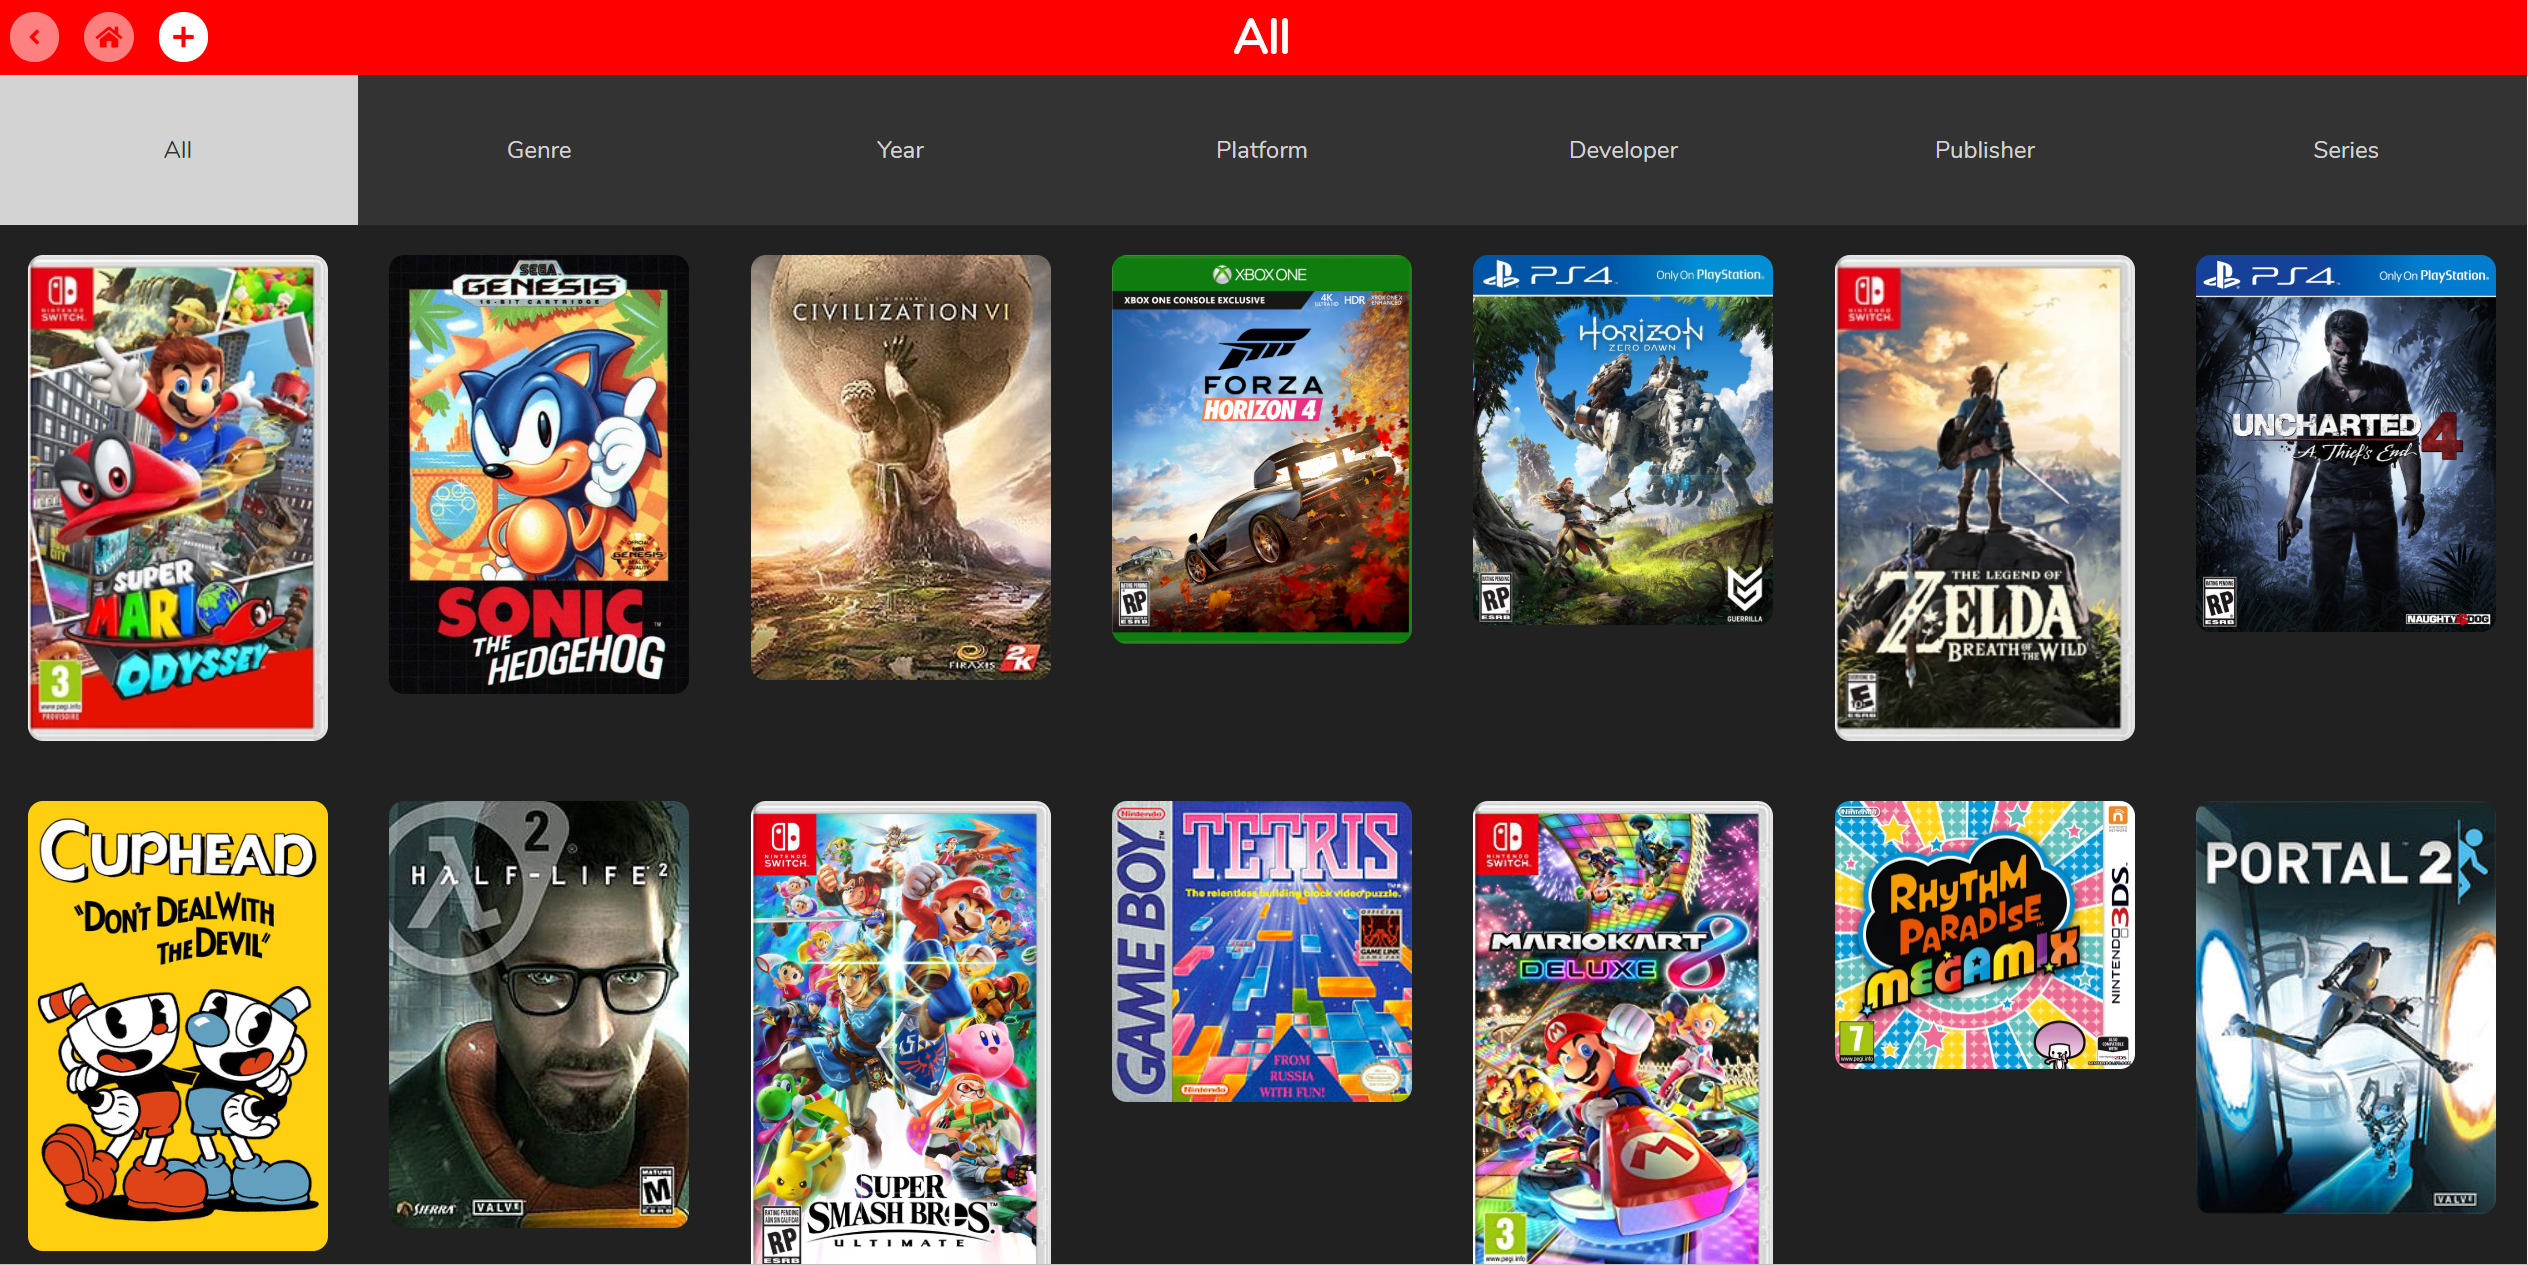
\includegraphics[width=\textwidth]{HomeScreen.PNG}
\caption[width=\textwidth]{Home Screen - An unfiltered list of games} \label{homeScreen}
\end{figure*}

\begin{figure*}
\includegraphics[width=\textwidth]{URLHierarchy.png}
\caption[width=\textwidth]{URL Hierarchy - The URL structure of the web app} \label{URLHierarchy}
\end{figure*}
		
\end{document}